%! Author = weiss
%! Date = 20.01.2025
\Author{\daAuthorThree}

    This chapter describes the use of a convex hull algorithm to define the boundaries of an area. It is a process of determin the outermost points of an area and joining them to create a border. This chapter also explains the fundamentals of the convex hull algorithm, other possible ways of calculating such a boundary and why we used this method in our project.

    \subsection{Purpose of Area Borders in the App}
    The convex hull algorithm is used in the app to define certain addresses which form the boundaries of an area. These boundaries are crucial to better organize and manage all areas which are assigned to all groups within the application. Below is a screenshot of the app that shows the highlighted borders of an area to visually demonstrate how these areas are shown within the app.

    \subsubsection{What are Border Addresses?}
    Border addresses are certain points that define the outer boundaries of an area. Furthermore, an area is defined by a set of addresses which get added to a certain area prior to the caroler campaign (Königskarten Aktion). Once the area is created, the convex hull algorithm can be applied on the list of addresses to find the border addresses. This border addresses just go around the perimeter of the area. Therefore, the outcome is a precise, convex shape that covers the entire area.
    
    \subsubsection{Why Do We Use Border Addresses?}
    Border addresses are important for a number of reasons. The give the visual definition of each area's boundaries, making it easy to manage and navigate through the different areas for admins and making it easier for each group to see the boundaries of their respective area. The use of the convex hull algorithm ensures that the boundary defined is the smallest convex shape possible that incorporates all the addresses in this area. The importance of the border addresses is outlined in the following points: \newline \newline
    \textbf{For the Admin:}
    \begin{enumerate}
        \item \textbf{Clear Visual Representation:} In the app interface, each area is shown in a different colour and border addresses are highlighted by a line which goes through all the border addresses of an area. This makes it easy for the admin to see where each area is and how big they are.
        \item \textbf{Efficient Area management:} By visualizing the areas with the border addresses highlighted, the admin can rapdily evaluate the boundaries of each area. Based on the result of each area's boundaries, the admin can remove or add addresses if necesssary. The management process is therefore improved by its flexibility. 
        \item \textbf{Better Decision Making:} The admin can make a well-informed decision about adding or removing addresses from an area by visually seeing how big an area is or how many addresses are in an area. Besides other factor, this information guarantees better decision making from the admin on how to distribute the addresses to each area.
    \end{enumerate}

    \textbf{For Each Group:}
    \begin{enumerate}
        \item \textbf{Clear Understanding of Area Boundaries:} The border addresses give guides of each group a clear idea of the addresses they are in charge of. Each group can also more easily see the boundaries of their area, which helps to avoid misunderstanding of where each group has to go and where they must not go.
        \item \textbf{Improved Navigation and Accuracy:} Guides are able to navigate better in their areas when they have a visual representation of their area. By keeping them within their area, this visual aid helps them avoid errors in for example visiting addresses from other areas. 
        \item \textbf{Increased Efficiency:} The guides are able to finish their work more quickly because the boundaries of each area are clearly marked. They can focus on their designated area and plan their routes to be as efficient as possible and to not cross any other areas in the process.
    \end{enumerate}

    \subsection{Overview of the Convex Hull Algorithm}
    The convex hull algorithm is a fundamental concept in computational geometry. On a two-dimensional system, it is used to find the smallest convex polygon that can hold a specific sets of points. Simply put, it determines the outer border or edge that surrounds each of the specified points. The convex hull, which is the outer boundary, is the tightest shape that can enclose every point without any spaces in between. \newline
    
    To better understand the concept, consider a set of points randomly placed on a flat surface. If a rubber band would be stretched around those points, it would form a shape that encloses the outermost points. This resulting shape is the convex hull, which is the smallest convex polygon that fully encloses all points. The image below shows exactly this process, with the points being surrounded by the convex hull. This gives a visual representation of the convex hull algorithm.
    \begin{figure} [H]
        \centering
        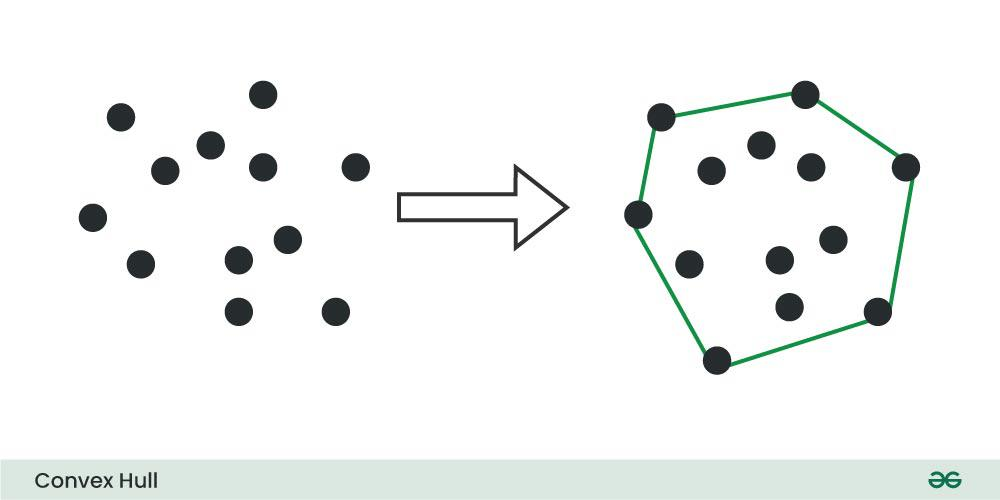
\includegraphics [width=1\textwidth] {images/andreas/areaBorders/convexHull.jpg}
        \caption{Process of the Convex Hull Algorithm}
        \cite{Andi:convexHullPic}
    \end{figure} 
    \blankLine 
    A convex polygon is a shape where all the corners point outward and there are no inward curves or sharp angles. To put it simply, if you draw a straight line between any two points inside the shape, it will always remain inside or on the shape's edge. This indicates that there are never any inward corners on the convex hull. In contrast, a concave polygon has atleast one or more inward curves where the interior angle is greater than 180 degrees. \newline
    To better visualize the difference, the image below shows that all the angles of the convex polygon have less than 180 degrees, therefore they are "pointy". However, on the concave polygon it is visible that the angles on top has more than 180 degrees, therefore the polygon has an inwards curve \autocite{Andi:convexPolygon}

    \begin{figure} [H]
        \centering
        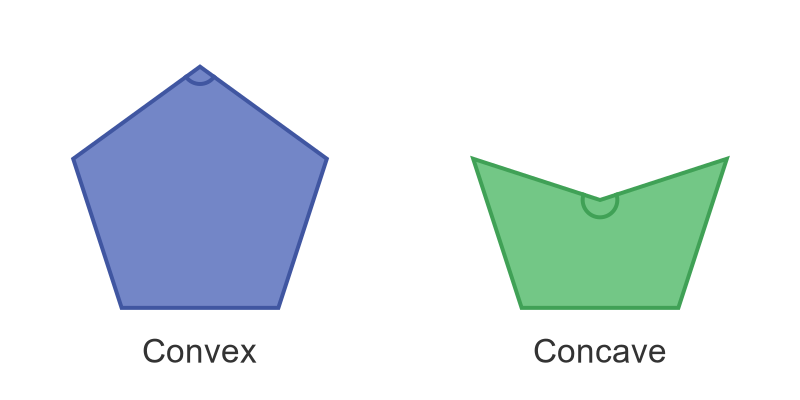
\includegraphics [width=1\textwidth] {images/andreas/areaBorders/convexConcave.png}
        \caption{Difference between a convex/concave polygon}
        \cite{Andi:concaveConvex}
    \end{figure}

    \subsubsection{Why Use the Convex Hull?}
    The convex hull algorithm si especially helpful for identifying a set of points' boundary and eliminating any extra points that fall inside it. In the cas of the addresses of each area, for example, the convex hull algorithm helps in defining the outermost boundaries that enclose these points in the smallest possible area. Whether in pathfinding, geographical mapping or other spatial analysis applications that demand distinct boundary limits, this procedure is crucial.

    \subsubsection{Types of Convex Hull Algorithms}
    The convex hull can be calculated using a variety of algorithms, with the most popualar being \textbf{Graham's Scan} and the \textbf{Monotone Chain algorithm}. Because of their effectiveness and capacity to manage sizable datasets, these algorithms have been widely adopted. \newline \newline

    \textbf{Graham's Scan Algorithm:} 
    \begin{itemize}
        \item Graham's Scan is a methods which was introduced in 1972 to find the convex hull of a set of points. The process starts by sorting the points based on the "polar angle" of each point relative to the bottom-most point. Simply speaking, the polar angle is the angle between a point and a reference direction which is often the horizontal axis (the x-axis).
        \item As soon as the points are sorted, the algorithm builds the convex hull by looking at each point in the sorted list. It moves from one point to the next, while going through each point it checks if the previous three points form a right or a left turn. As soon as a right turn is detected, the last point is removed, because it would create an inward curves in the shape, which would then result in a concave hull and not a convex hull. The algorithm continues with this until the hull is fully formed.
        \item The time it takes to run the Graham's Scan is \textbf{O(N log N)}, with N as the total number of points. Therefore, the required time grows reasonably with a larger dataset which makes it efficient for moderately large sets of points.
    \end{itemize} 
    \blankLine 
    \textbf{Monotone Chain Algorithm:}
    \begin{itemize}
        \item The Monotone Chain algorithm was introduced in 1979 and is antoher efficient way to calculate a convex hull. It begins by soirting the points based on their horizontal position (x-coordinate), from the leftmost to the rightmost.
        \item The algorithm then makes two steps to construct the convex hull. First is the upper hull and then the lower hul. The algorithm goes through the sorted list of points, adding them to the hull and ensures that each new point does not cause a inward curve by checking whether the last three points form a right or left turn, just like in Graham's Scan.
        \item The run time is the same as the Graham's Scan with \textbf{O(N log N)}, which makes it well-suited for larger datasets.
    \end{itemize} \autocite{Andi:typesOfConvexHullAlgos, Andi:convexHullPic}

    \subsubsection{Key concepts in the Convex Hull Algorithm}
    The convex hull algorithm has a number of key concepts, all of which are essential to guaranteeing the algorithm's accuracy and effectiveness. \newline \newline
    \textbf{Orientation:}
    \begin{itemize}
        \item This is a reference to the relative orientation of three consecutive points. The convex hull algorithm determines wether to add the next point to the hull based on the orientation of a triplet of points. There are three possible orientations for the points: clockwise, anticlockwise and collinear. Only if the points are oriented counterclockwise, should the point be part of the hull. Otherwise it should be discarded.
    \end{itemize}

    \textbf{Polar Angle Sorting:}
    \begin{itemize}
        \item A key step in convex hull algorithms is sorting the points according to their polar angle relative to a fixed point which is usually the lowest or leftmost point. By sorting the points, this process guarantees that they are processed in a way that minimises computing resources during hull construction.
    \end{itemize}

    \textbf{Stack Operations:}
    \begin{itemize}
        \item Convex hull algorithms often use a stack data structure to keep track of all points that are currently part of the hull. To guarantee that only the outermost points stay in the stack, points are added and removed according to their orientation relative to their earlier points.
    \end{itemize}

    \textbf{Convexity:}
    \begin{itemize}
        \item The convexity of the polygon that is formed by a convex hull algorithm ensures that there are no inward curves. This is crucial because the convex hull represents the smallest possible polygon that does not have any concave edges or inward curves.
    \end{itemize} \autocite{Andi:keyConcepts}

    \subsection{Use Cases of the Convex Hull in Industry}
    The ability if the convex hull algorithm to define boundaries of a complex dataset in an efficient way makes it widely used across a variety of fields. Convex hulls offer crucial tools for examining spatial relationships, visualising data and resolving optimisation issues in a variety of fields. Here are some fields that use this algorithm. \newline \newline
    \textbf{Geographical Mapping}
    \begin{itemize}
        \item In geographic mapping, convex hulls are used to define the borders of regions. For example, while mapping a region with multiple data points, such as cities or landmarks, the convex hull helps outline the area that encloses all the points. This makes it easier to visualize and analyze the overall shape of a region which helps with urban planning, resource management and environmental studies.
    \end{itemize}
    \textbf{Image Processing and Computer Vision}
    \begin{itemize}
        \item Convex hulls are used in image processing to determine the shape of an object. THis is helpful for tasks like object recognition, where the convex hull helps defining and object's boundaries which improves detection. It makes it easier for algorithms to process and categorise objects in an image by reducing complex shapes to convex polygons.
    \end{itemize}
    \textbf{Computational Geometry}
    \begin{itemize}
        \item Convex hulls are crucial in computational geometry for solving issues such as determining the smallest polygon possible that contains a set of points. This has uses in fields like pattern recognition. By providing this convex hull, algorithms can concentrate on the outermost points and ignore the inner one which lowers processing cost.
    \end{itemize}
    \textbf{Animal Behavior}
    \begin{itemize}
        \item In ethology, the study of animal behavior, convex hulls are used to identify and anmial's home range. The convex hull gives the estimated area an animal needs to be provided with for its inhabitat. In ecological sutdies, this approach is helpful for tracking animal movement patterns, determining territories and keeping an eye on endangered species.
    \end{itemize}
    \textbf{Astronomy and Astrophysics}
    \begin{itemize}
        \item Astronomers utilise convex hulls to define the limits of star clusters and other celestial bodies. Scientists can determine a cluster's outer limit by looking at the convex hull of stars which helps them study things like galactic formation, star density and gravitational impacts in space.
    \end{itemize}
    \autocite{Andi:irlApplication}

    \subsection{Alternate Methods for Area Border Calculation}
    The convex hull algorithm is a widely used approach for calculating area boundaries. However, there are other methods that may be more suitable depending on the application requirements. These alternative methods offer different ways to calculate area boundaries with varying levels of complexity and accuracy. \newline \newline
    \textbf{Minimum Bounding Box (MBB)}
    \begin{itemize}
        \item The simplest technique for calculating area boundaries is the MBB. It determines the smallest rectangle that completely encloses a specified set of points. The Edges of the box is normally aligned with the coordiante axes, which makes it efficient with the computing resources and easy to implement. Applications like spatial indexing in databases and image processing use this technique. However, because it does not consider things like concavities and irregularities in the point distribution which may lead to the MBB not always correctly reflecting the data. The Picture below shows a figure which visualizes the difference between the MBB and the convex hull. The convex hull is the gray inner are and the outer line is the MBB. This shows that the convex hull is more precise. \autocite{Andi:mbb}
    \end{itemize} 

    \begin{figure} [H]
        \centering
        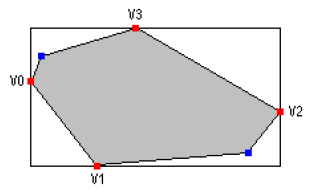
\includegraphics [width=.55\textwidth] {images/andreas/areaBorders/mbb.png}
        \caption{Difference between MBB and Convex Hull}
        \cite{Andi:mbbPic}
    \end{figure}

    \textbf{Alpha Shapes}
    \begin{itemize}
        \item By adding a new parameter, $\alpha$, that controls how closely the boundary should attach to the specified point, alpha shapes offer a more flexible method of defining area bounds. This approach is more accurate than the convex hull for irregular shapes because it may caputre concave features by decreasing this new parameter $\alpha$. This method is especially helpful in fields like shape recognition, molecular modeling and terrain analysis where precisely recording complex boundaries is crucial. Choosing an appropriate $\alpha$ value is the main challenge with Alpha Shapes as different datasets may require different levels of precision. In the picture below there is the difference between convex hull and Alpha Shapes. It shows that in this case the Alpha Shapes actually make a better job than the convex hull. \autocite{Andi:alphaShape}
    \end{itemize} 

    \begin{figure} [H]
        \centering
        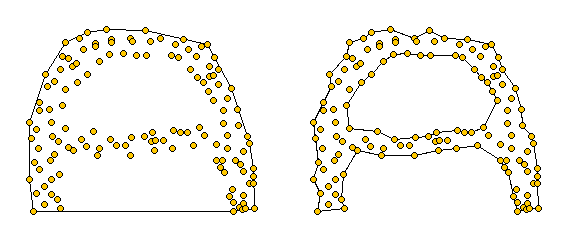
\includegraphics [width=.75\textwidth] {images/andreas/areaBorders/alphaShapePic.png}
        \caption{Difference between Alpha Shape and Convex Hull}
        \cite{Andi:alphaShapePic}
    \end{figure}

    \textbf{Delaunay Triangulation}
    \begin{itemize}
        \item Delaunay Triangulation is a method that makes a mesh of triangles which connect a set of points while maximizing the minimum angle of each traingle. This ensures a well-formed structure. A border can be roughly approximated by using the Triangulation's outside edges, especially when pairing this method with techniques like Alpha Shapes. THis method is mostly used in geographic information systems (GIS). While it provides a more structured representation of an area, it often requires post-processing to extract a meaningful boundary.
    \end{itemize} \autocite{Andi:DT}

    \begin{figure} [H]
        \centering
        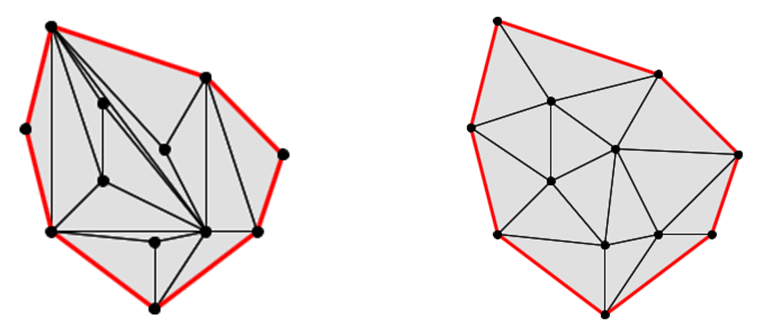
\includegraphics [width=.75\textwidth] {images/andreas/areaBorders/dtPic.png}
        \caption{Mesh of Triangles from Delaunay Triangulation}
        \cite{Andi:dtPic}
    \end{figure}

    \subsection{Rationale for Choosing the Convex Hull Method}
    Accuracy, computational efficiency and implementation ease had to be balanced when choosing a method for identifying area borders. The convex hull was selected as the best strategy for our application after a number of approaches were taken into consideration. \newline
    One major reason for this choice was that the convex hull method was precise enough in comparison with more complex methods like the alpha shapes. Since our application did not need such fine control, the additional complecity of alpha shapes was unnecessary. \newline
    Furthermore, the convex hull approach offers a significant advantage in terms of speed. It enables quick computing in comparison to other methods which makes it ideal for our application as our resources where somewhat limited for the border addresses. \newline
    Finally, our choice was significantly influenced by ease of implementation. The convex hull approach does not require a lot of parameter adjusting, is well-documented, and is simple to incorporate. This made it a practical choice which allows for a reliable and efficient solution without adding unnecessary complexity. \newline
    A fair balance between accuracy and efficiency was achieved by selecting the convex hull method which allowed area borders to be calculated quickly whil still providing a clear visual representation of each area.

    \subsection{Integration of the Algorithm into the Backend}
    The convex hull algorithm is implemented within the backend as a part of the service class which analyses an area's allocated addresses to identify its boundaries. The frontend can request and use the calculated border addresses thanks to this functionality which is made available through a dedicated route. \newline
    As soon as a request is made to the route, the service class gets the area for which the border addresses are needed. The program then retrieves all the addresses in the respective area which then get processed by the convex hull algorithm. This then determines the smallest convex shape that encloses all points. The result list of all border addresses are then returned as a response to the frontend, where they are getting used for visualization and management. \newline
    The server-side calculation laod is effectively managed by implementing the convex hull calculation directly in the backend, guaranteeing reliable and consistent results on all client devices.

    \newpage